\documentclass{article}

\usepackage{graphicx}
\usepackage{tikz}
\usepackage{tikzsymbols}
\usetikzlibrary{calc,patterns,shapes.geometric}
\pagestyle{empty}
\usepackage[margin=0pt]{geometry}
\geometry{papersize={14in,12in}}

\def\centerarc[#1](#2)(#3:#4:#5){\draw[#1] ($(#2)+({#5*cos(#3)},{#5*sin(#3)})$) arc (#3:#4:#5);}

\begin{document}
	\begin{figure}
		\centering
		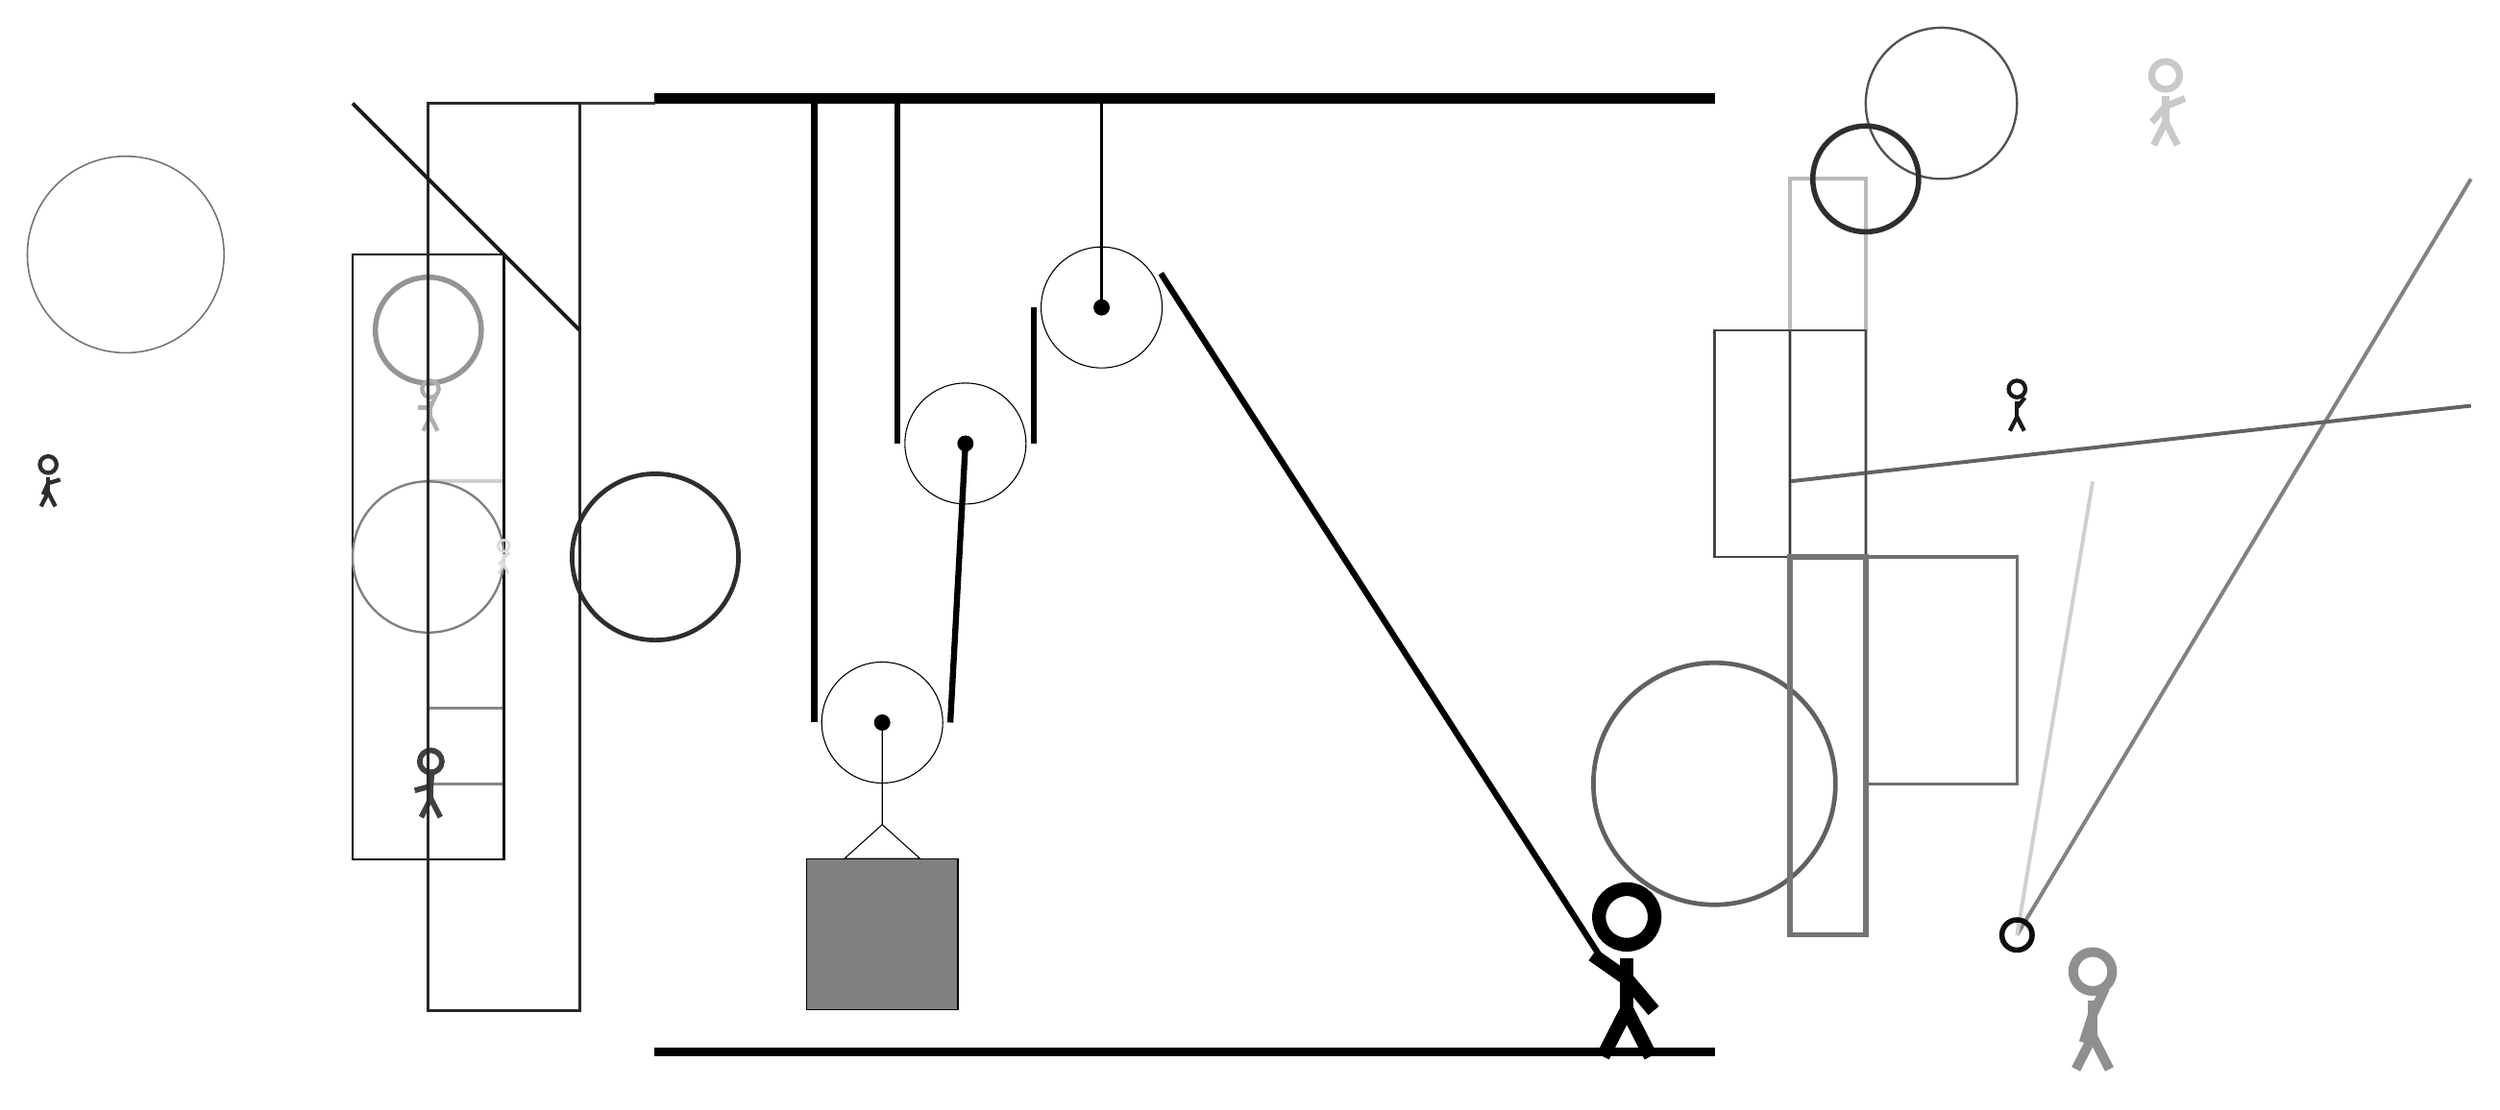
\begin{tikzpicture}
			%%%%% START %%%%%
			
			\draw[fill=black] (-2, 9) rectangle (12, 9.125);
			
			\draw (1, 0.81) circle (0.8);
			\draw[fill=black] (1, 0.81) circle (0.1);
			
			\draw (2.1, 4.5) circle (0.8);
			\draw[fill=black] (2.1, 4.5) circle (0.1);
			
			\draw (3.9, 6.3) circle (0.8);
			\draw[fill=black] (3.9, 6.3) circle (0.1);
			\draw[thick] (3.9, 6.3) -- (3.9, 9);
			
			\draw (1, 0.81) -- (1, -0.54) -- (0.5, -0.99) -- (1.5, -0.99) -- (1, -0.54);
			\draw[fill=black!50] (0, -0.99) rectangle (2, -2.99);
			
			\draw [line width=0.6mm, color=black!62](12, 0) circle (1.6);
			
			\draw[line width=0.5mm, color=black!19](-4, 4) -- (-5, 4);
			\draw[line width=0.5mm, color=black!49](16, -2) -- (22, 8);
			\draw[line width=0.5mm, color=black!19](16, -2) -- (17, 4);
			
			\draw [line width=0.6mm, color=black!82](-2, 3) circle (1.1);
			\draw [line width=0.7mm, color=black!42](-5, 6) circle (0.7);
			\draw[line width=0.4mm, color=black!47] (-4, 1) rectangle (-5, 0);
			\node[line width=0.7mm, color=black!32] at (-5, 5) {\Strichmaxerl[3][0][65]};
			\draw[line width=0.3mm, color=black!97] (-4, -1) rectangle (-6, 7);
			\draw[line width=0.5mm, color=black!27] (13, 8) rectangle (14, -2);
			
			\node[line width=0.6mm, color=black!90] at (16, 5) {\Strichmaxerl[3][90][52]};
			\draw[line width=0.5mm, color=black!61](13, 4) -- (22, 5);
			\draw[line width=0.2mm, color=black!78] (13, 6) rectangle (13, 1);
			
			\draw [line width=0.3mm, color=black!68](15, 9) circle (1.0);
			\draw[line width=0.4mm, color=black!99] (12, 3) rectangle (12, 3);
			\node[line width=0.6mm, color=black!44] at (17, -3) {\Strichmaxerl[7][72][65]};
			
			\node[line width=0.5mm, color=black!82] at (-10, 4) {\Strichmaxerl[3][66][16]};
			\draw[line width=0.4mm, color=black!79] (-4, 9) rectangle (-2, 9);
			\draw[line width=0.4mm, color=black!56] (14, 0) rectangle (16, 3);
			\node[line width=0.5mm, color=black!75] at (-5, 0) {\Strichmaxerl[4][15][86]};
			\draw[line width=0.3mm, color=black!72] (12, 3) rectangle (14, 6);
			
			\draw [line width=0.7mm, color=black!82](14, 8) circle (0.7);
			\draw [line width=0.3mm, color=black!50](-5, 3) circle (1.0);
			\draw [line width=0.7mm, color=black!95](16, -2) circle (0.2);
			\node[line width=0.3mm, color=black!21] at (18, 9) {\Strichmaxerl[5][49][22]};
			
			\draw[line width=0.4mm, color=black!84] (-3, -3) rectangle (-5, 9);
			\draw[line width=0.5mm, color=black!90](-3, 6) -- (-6, 9);
			\node[line width=0.7mm, color=black!15] at (-4, 3) {\Strichmaxerl[2][55][43]};
			
			\draw [line width=0.2mm, color=black!55](-9, 7) circle (1.3);
			
			\draw[line width=0.7mm, color=black!54] (14, 3) rectangle (13, -2);
			
			\draw[line width=0.8mm] (0.1, 9) -- (0.1, 0.81);
			\centerarc[line width=0.8mm](1, 0.81)(180:360:0.9);
			\draw[line width=0.8mm](1.9, 0.81) -- (2.1, 4.5);
			\draw[line width=0.8mm] (1.2, 9) -- (1.2, 4.5);
			\centerarc[line width=0.8mm](2.1, 4.5)(180:360:0.9);
			\draw[line width=0.8mm](3.0, 4.5) -- (3.0, 6.3);
			\centerarc[line width=0.8mm](3.9, 6.3)(30:180:0.9);
			\draw[line width=0.8mm] (4.683, 6.75) -- (10.5, -2.3);
			
			\node at (10.8, -2.5) {\Strichmaxerl[10][-35][-50]};
			
			\draw[fill=black] (-2, -3.5) rectangle (12, -3.6);
			
			%%%%% END %%%%%
		\end{tikzpicture}
	\end{figure}	
\end{document}